\documentclass[aspectratio=169,10pt]{beamer}
\usepackage[T1]{fontenc}
\usepackage{amsmath,amssymb,graphicx}
\definecolor{ink}{HTML}{203550}
\definecolor{teal}{HTML}{008783}
\setbeamercolor{frametitle}{fg=ink}
\setbeamercolor{structure}{fg=teal}
\setbeamercolor{normal text}{fg=ink,bg=white}
\setbeamertemplate{navigation symbols}{}
\setbeamertemplate{footline}{\hfill\scriptsize AKO (2026)\quad\insertframenumber/\inserttotalframenumber\hspace{4mm}\vspace{2mm}}
\setbeamersize{text margin left=8mm,text margin right=8mm}
\newcommand{\src}[1]{\vfill{\tiny\color{gray}#1}}
\title{AI, Human Cognition and Knowledge Collapse}
\subtitle{Why better advice can weaken collective learning}
\author{fgalarzac\quad |\quad AI-Econ-Modeling}
\date{Acemoglu, Kong \& Ozdaglar (2026)\quad NBER WP 34910}
\begin{document}
\begin{frame}[plain]
\titlepage
\centering\small\href{https://github.com/fgalarzac/ai-04-acemoglu}{github.com/fgalarzac/ai-04-acemoglu}
\medskip

\scriptsize Course-linked MIT: May 5, 2026 (69 pages); NBER cross-check: September 10, 2026.\\
Unrefereed working paper. Labels distinguish PAPER, DERIVATION and INTERPRETATION.
\end{frame}

% Target speaking time: 50 seconds.
\begin{frame}{1. The paper and the agent's problem}
\textbf{PAPER:} Learning jointly supplies private context and public knowledge.\\
AI replaces the private incentive; the public benefit goes to future cohorts.
\[
\max_{e\ge0}\ f(0,0)+\Delta_GG(X)+\Delta_XG(X)G(Y)-\frac{e^\alpha}{\alpha},
\qquad Y=\sigma^{-2}+\lambda_Ie+\tau_A.
\]
\[
G(q)=2\Phi(\sqrt q)-1,\quad g(q)=\frac{\phi(\sqrt q)}{\sqrt q},\qquad
\boxed{e^{\alpha-1}=\Delta_X\lambda_IG(X)g(Y)}\quad(X>0).
\]
\begin{itemize}
\item $\Delta_I=0$, $\Delta_X>0$, $\Delta_G\ge0$, $\Delta_G+\Delta_X=1$; $\alpha>1$.
\item Medical knowledge + patient symptoms; financial knowledge + risk tolerance.
\item Convex costs give a unique optimum. At $X=0$, the optimum is $e=0$.
\end{itemize}
\src{PAPER: §§3.1, 3.3, 3.5. NBER uses $\alpha$; MIT uses $\varepsilon=1/(\alpha-1)$.}
\end{frame}

% Target speaking time: 40 seconds.
\begin{frame}{2. Observation 1: two signs, one boundary}
\textbf{DERIVATION, matching PAPER §3.4:} for $X>0$,
\[
U_{eX}=\Delta_X\lambda_Ig(X)g(Y)>0,
\qquad
U_{e\tau_A}=\Delta_X\lambda_IG(X)g'(Y)<0,
\]
\[
g'(Y)=-\frac{1+1/Y}{2}g(Y)<0.
\]
\begin{itemize}
\item More public knowledge raises the value of learning one's own context.
\item AI supplies the same private precision; diminishing returns crowd out effort.
\item At $X=0$: $e=0$, $U_{e\tau_A}=0$; $g(X)$ is singular at zero.
\end{itemize}
\medskip
\textbf{Verdict:} strict interior inequalities need a boundary qualification.\\
\textbf{Issue correction:} §2 is Related Literature; the static model is in §3.
\src{PAPER: Observation 1 and footnote in §3.5. Boundary statements: DERIVATION.}
\end{frame}

% Target speaking time: 60 seconds.
\begin{frame}{3. Main result: replenishment versus crowd-out}
\[
X_t\ \longrightarrow\ e_t\ \longrightarrow\ E_t=Ie_t\ \longrightarrow\
X_{t+1}=\frac{X_t+\lambda_GIe_t}{1+\Sigma^2(X_t+\lambda_GIe_t)}.
\]
\small
\textbf{Baseline conditions:} Assumption 1; power cost; atomistic short-lived Bayesian agents;
Gaussian signals; fixed $I,\lambda_I,\lambda_G,\Sigma^2,\sigma^{-2}>0$;
finite $\tau_A\ge0$; linear public learning, no synthetic input.
\begin{itemize}
\item $\alpha-1>1/4$ ($\varepsilon<4$): zero unstable; one positive stable state.
Every $X_0>0$ converges to it.
\item $0<\alpha-1<1/4$ ($\varepsilon>4$): zero stable. Below $\tau_A^c$, an unstable
$\bar X_m$ separates collapse from $\bar X_h$. Above $\tau_A^c$, all paths collapse.
\item $\tau_A^c$ may be zero; $X_0=\bar X_m$ stays there.
At $\tau_A=\tau_A^c>0$, Appendix A.4 retains a tangency. $\varepsilon=4$ is a separate boundary.
\end{itemize}
\textbf{PAPER intuition:} chosen effort near zero is of order $X^{\varepsilon/2}$; maintenance needs $X^2$.
\src{PAPER: Lemma 2, Propositions 3 and 5; Appendix A.4--A.6, Lemmas A-1--A-4. Explained, not re-proved.}
\end{frame}

% Target speaking time: 45 seconds.
\begin{frame}{4. What I did: visualize the dynamics}
\centering\small Left: vary $\alpha$, $\tau_A=0$.\qquad Right: vary $\tau_A$, $\alpha=1.2$.\\
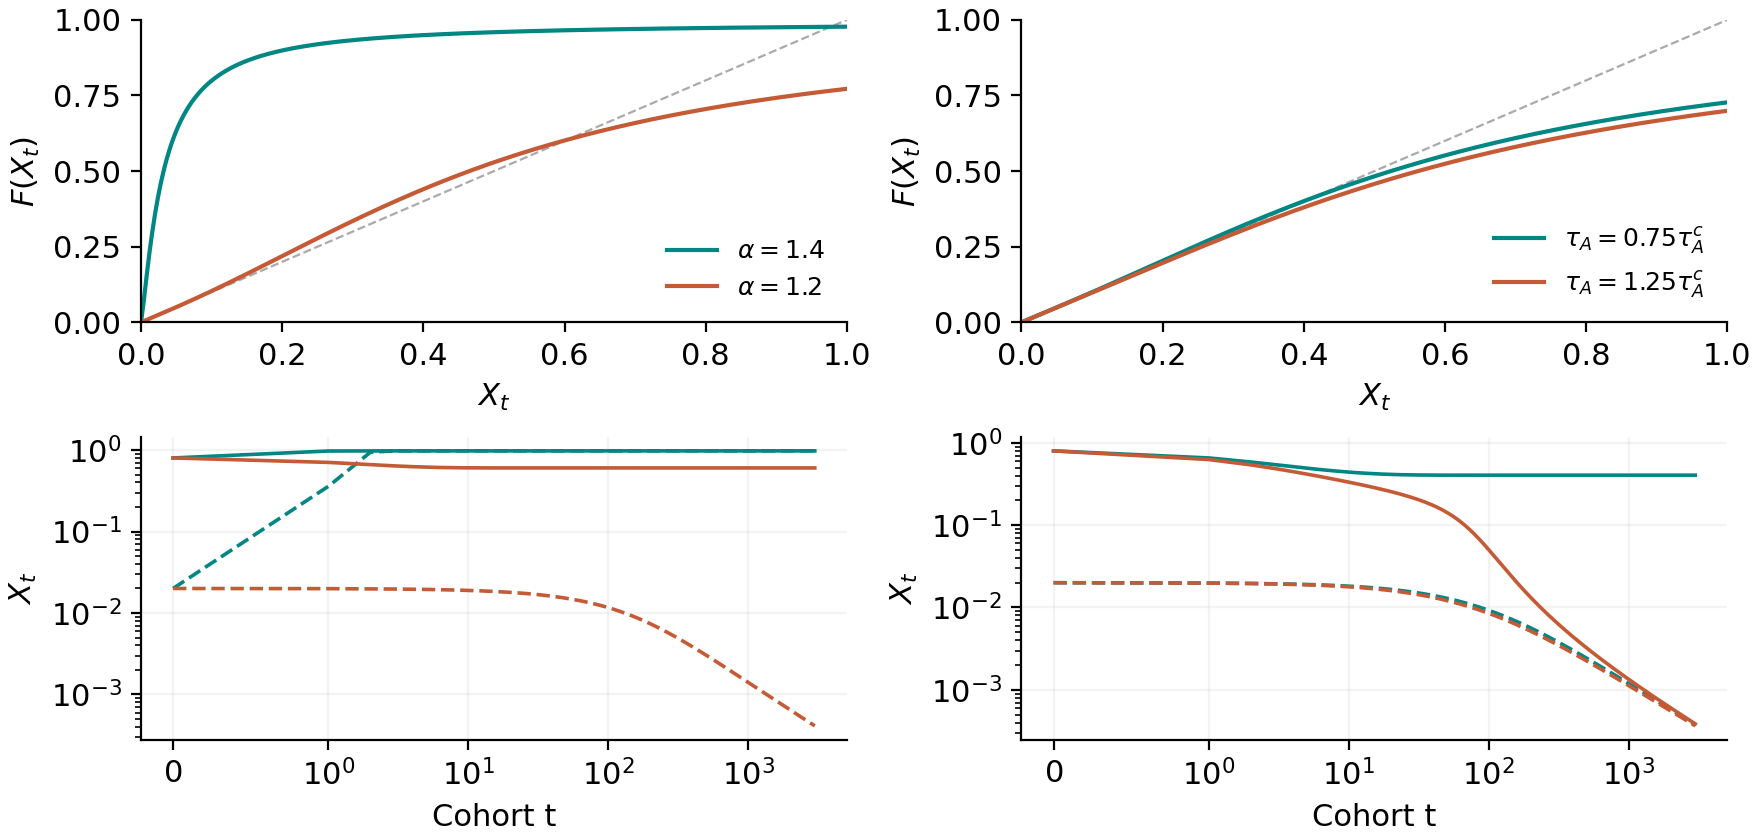
\includegraphics[width=.95\textwidth,height=4.8cm,keepaspectratio]{figures/slide_overview.png}
\par\raggedright
\scriptsize
$\lambda_I=\lambda_G=\Sigma^2=\Delta_X=1$, $I=1000$, $\sigma^{-2}=0.5$, $\Delta_G=\Delta_I=0$;
$X_0=0.02,0.8$. 3,000 steps; time paths use log scales.\par
Computed $\tau_A^c\approx0.06698$. Solid paths: $X_0=0.8$; dashed: $X_0=0.02$.
Full cobwebs and the parameter-specific $\alpha=1.25$ case are in the README. Small values are not zero.
\src{Numerical illustration of PAPER Figures 1--2, not a new result. FOC, map, crowd-out and root-count checks pass.}
\end{frame}

% Target speaking time: 50 seconds.
\begin{frame}{5. Where I did not trust the AI: welfare}
\textbf{Claim checked:} ``More accurate AI must increase welfare.''
\[
\frac{d\bar U^+}{d\tau_A}=
\underbrace{\Delta_XG(\bar X_h)g(\bar Y_h)}_{\text{direct information gain}}
+\underbrace{g(\bar X_h)[\Delta_G+\Delta_XG(\bar Y_h)]\frac{d\bar X_h}{d\tau_A}}_{\text{indirect knowledge loss}}.
\]
\begin{itemize}
\item Private-effort terms cancel by the envelope theorem; the public loss remains.
\item Under $\sigma^{-2}\ge\sqrt2-1$: single peak on the high branch, possibly at zero AI.
\item An interior peak needs the direct gain to dominate initially.
\item In the elastic regime, basin selection can cause an additional welfare drop.
\end{itemize}
\textbf{Verdict:} reject a blanket monotonicity claim; do not promise an interior optimum.
\src{PAPER: Propositions 10--11 (high branch must exist), §§4.1--4.3; envelope calculation: DERIVATION.}
\end{frame}

% Target speaking time: 35 seconds; total approximately 5 minutes including title.
\begin{frame}{6. Assumption audit and honest limits}
\begin{columns}[T]
\column{.65\textwidth}
\small
\textbf{PAPER §5 actually changes:}
\begin{itemize}
\item §5.1: aggregation $I(\tau_A)$.
\item §5.2: synthetic public precision.
\item §5.3: public learning $e^\beta$.
\end{itemize}
\textbf{Retained:} $\Delta_I=0$, $\Delta_X>0$, power cost.\\
The unrelaxed production restriction is that context information alone has no value.
\medskip

\textbf{OPEN QUESTIONS:} standalone context value; varying cost elasticity; contribution rewards.
\medskip

\textbf{INTERPRETATION:} a conditional theoretical mechanism, not an empirical forecast.
\column{.32\textwidth}
\centering
\IfFileExists{hand/derivation.jpg}{
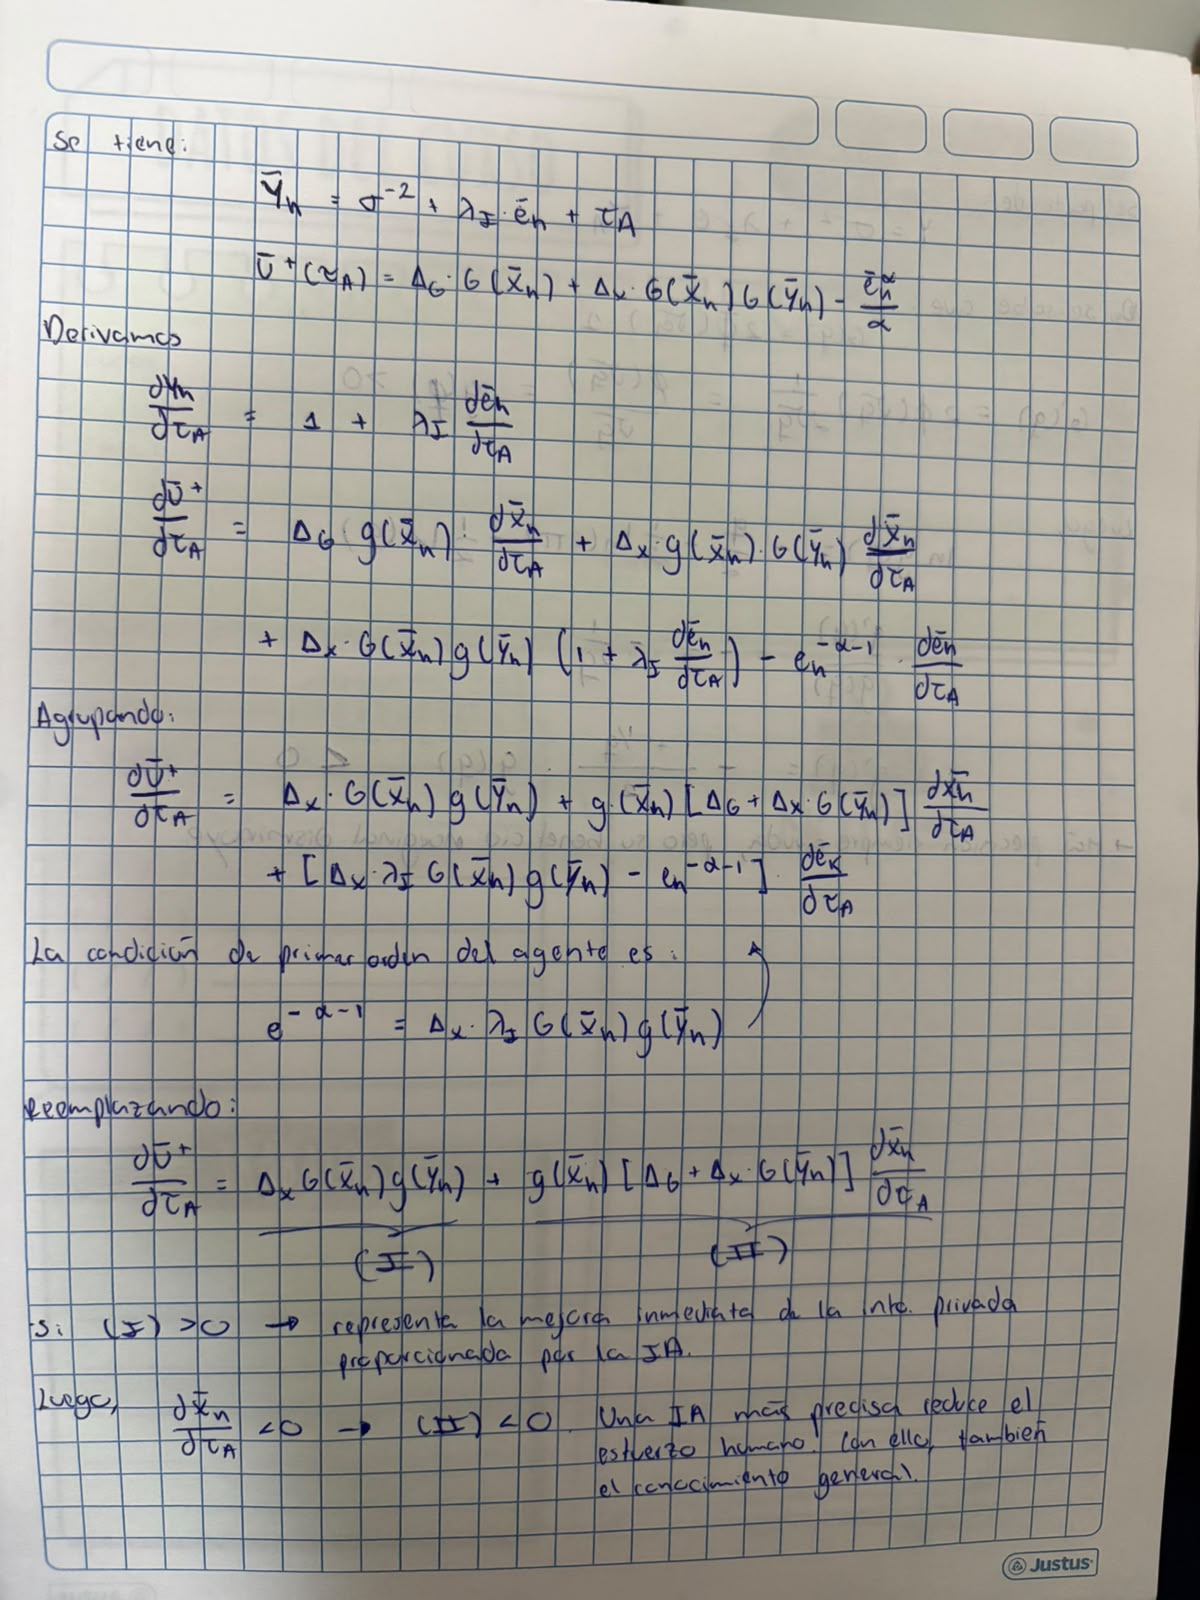
\includegraphics[width=\linewidth,height=3cm,keepaspectratio]{hand/derivation.jpg}
\par\scriptsize User-supplied handwritten work; caption to be confirmed.
}{
\fbox{\parbox[c][2.8cm][c]{.88\linewidth}{\centering\small Handwritten photo\\pending from user\\\medskip\scriptsize hand/derivation.jpg}}
\par\medskip\scriptsize No handwritten verification is claimed yet.
}
\end{columns}
\src{Section 5 and Appendix B checked. Candidate extensions are new relative to this paper only.}
\end{frame}
\end{document}
